% This file was converted to LaTeX by Writer2LaTeX ver. 0.5
% see http://www.hj-gym.dk/~hj/writer2latex for more info
\documentclass{article}
\usepackage[ascii]{inputenc}
\usepackage[T1]{fontenc}
\usepackage[english]{babel}
\usepackage{amsmath,amssymb,amsfonts,textcomp}
\usepackage{color}
\usepackage{array}
\usepackage{hhline}
\usepackage{hyperref}
\hypersetup{pdftex, colorlinks=true, linkcolor=blue, citecolor=blue, filecolor=blue, pagecolor=blue, urlcolor=blue, pdftitle=, pdfauthor=qiangwz, pdfsubject=, pdfkeywords=}
\usepackage[pdftex]{graphicx}
% List styles
\newcommand\liststyleLi{%
\renewcommand\theenumi{\arabic{enumi}}
\renewcommand\theenumii{\arabic{enumii}}
\renewcommand\theenumiii{\arabic{enumiii}}
\renewcommand\theenumiv{\arabic{enumiv}}
\renewcommand\labelenumi{\theenumi.}
\renewcommand\labelenumii{\theenumii.}
\renewcommand\labelenumiii{\theenumiii.}
\renewcommand\labelenumiv{\theenumiv.}
}
% Page layout (geometry)
\setlength\paperwidth{8.5in}
\setlength\paperheight{11in}
\setlength\voffset{-1in}
\setlength\hoffset{-1in}
\setlength\topmargin{0.7874in}
\setlength\oddsidemargin{0.7874in}
\setlength\textheight{9.4251995in}
\setlength\textwidth{6.9251995in}
\setlength\footskip{0.0cm}
\setlength\headheight{0cm}
\setlength\headsep{0cm}
% Footnote rule
\setlength{\skip\footins}{0.0469in}
\renewcommand\footnoterule{\vspace*{-0.0071in}\setlength\leftskip{0pt}\setlength\rightskip{0pt plus 1fil}\noindent\textcolor{black}{\rule{0.25\columnwidth}{0.0071in}}\vspace*{0.0398in}}
% Pages styles
\makeatletter
\newcommand\ps@Standard{
  \renewcommand\@oddhead{}
  \renewcommand\@evenhead{}
  \renewcommand\@oddfoot{}
  \renewcommand\@evenfoot{}
  \renewcommand\thepage{\arabic{page}}
}
\makeatother
\pagestyle{Standard}
\title{}
\begin{document}
{\centering
Towards cross-domain authentication and standardized attribute-based
authorization for ARC grid middleware
\par}


\bigskip

Abstract-{}-


\bigskip


\bigskip


\bigskip

\liststyleLi
\begin{enumerate}
\item {\centering
Introduction
\par}


\bigskip
\end{enumerate}

\bigskip


\bigskip

{\centering
2. ARC grid middleware 
\par}

ARC(Advanced Resource Connector) is an open source grid middleware
solution released under GPL licence. ARC middleware initially aimed at
developing a grid middleware which provides characteristics such as
self-organized, fault-tolerant, non-intrusive, easy-management [fgcs
ARC paper]. \ Now \ the classic version of ARC provides grid services
such as grid job submission and management, resource characterization,
resource aggregation and discovery, basic data management, integration
of grid security solution, etc. Classic ARC has been deployed and used
in production environment, and been one of the mainly deployed grid
middlewares in Europe.

The new generation of ARC is funded by KnowARC project, and based on the
functionality and capabilities of the classic ARC middleware, it aims
at implementing a service-oriented middleware which will provide higher
levels of resource and user abstracting through well-defined web
service interface [Design document] in order to provide
interoperability with other service-based grid middlewares, as well as
other Web Service compatible applications.

As the key part of the implementation of new ARC middleware, there is a
lightweight web service container called HED (Hosting Environment
Daemon) which provides a host place for various services in application
level, as well as a host place for a bunch of components to support
flexible, interoperatible, and efficient communication mechanism. The
whole design of the HED is built around the idea of flexibility and
modularity, which means for the developer, he can easily concentrate on
the application level Web Service implementation by only using the core
minimum amount of components if he only would do application level
development, or he can easily concentrate on the middleware level
implementation such as supporting another communication protocol or
implementing authentication mechanism by using the core minimum amount
of components and external dependencies; also for the deployer, he can
easily configure and deploy the middleware and application for
different kinds of requirements without being bothered to know much
about the implementation.

{\centering
Figure 1. The architecture of Host Environment Daemon
\par}

\begin{center}
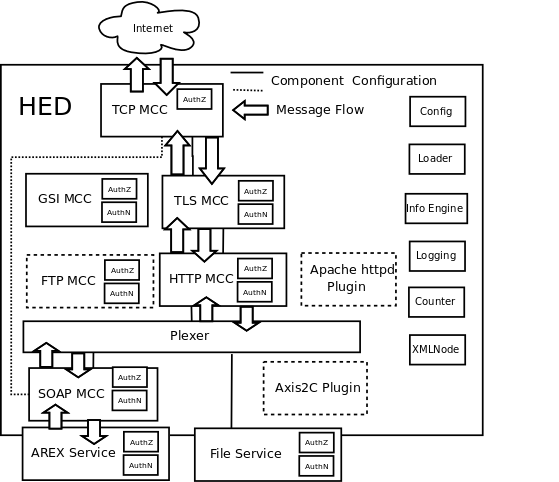
\includegraphics[width=4.0673in,height=3.1047in]{Secpaper-img1.png}
\end{center}
The architecture of the Host Environment Daemon is illustrated as Figure
1. In general, there are a few \ components called MCC (Message Chain
Components) which are in charge of processing different messages for
different protocol levels. For instance, as shown in the example
message flow, HTTP MCC will process secure socket stream from TLS MCC
to generate output HTTP message to SOAP MCC, and also process SOAP
documentation from SOAP MCC to generate HTTP message to TLS MCC. 

Two examples of MCC components configuration in Figure 1 shows MCC are
configurable: real line shows SOAP over HTTPS (HTTP over TLS), while
dotted line shows SOAP directly over TCP. Service administrator can
configure the MCCs according to his requirement, such as the
interoperability requirement with the other part. For instance, the
later configuration is compatible to WSE (Web Services Enhancement for
.NET) {\textquotesingle}s SOAP message mechanism (see
WSE{\textquotesingle}s \textit{SoapSender} and \textit{SoapReceiver}).
Another configuration could be SOAP over HTTPG (HTTP over GSI) which
can be user to interoperate with some service based on HTTPG such as
SRM (Storage Resource Manager) [ref] service. The easily configurable
characteristics shows the flexibility of HED in terms of protocol
supporting.

Because in the current state HED mostly provides modules for building
SOAP based Web Services, it is easy to think that HED is just another
Web Services development framework like Axis, gSOAP, XFire or any other
out of the numerous implementations. Instead, the idea of HED is to
provide framework for gluing functionalities and not a
re-implementation of various standards. Effectively that means if
Apache httpd web server is considered by developers as necessary for
serving as front-end to services there could be plugin code written
which places Apache2 into a chain of other plugins of the HED, the same
for the Apache Axis SOAP implementation, as shown in Figure 1.

Even though the external solutions like Axis and Apache httpd can be
used for protocol supporting, \ two protocols are completely developed
in HED to support HTTP and SOAP in order to make the solution
lightweight and needed an implementation of those supported protocols
that is both simple and lightweight. However external solutions are
used whenever is appropriate - as in the case of TLS (openssl is used),
GridFTP (GridFTP API is used), LDAP and some other cases, this
principle applies to Axis and Apache httpd if we used the API from
those solution to implement the plugins for supporting SOAP and HTTP
protocol. 


\bigskip


\bigskip


\bigskip

3. Cross-domain authentication and Single Sign-On


\bigskip

\ \ Community based authentication: Utilizing Shibboleth IdP


\bigskip

\ \ Short-lived certificate service


\bigskip

\ \ Certificate delegation service


\bigskip

\ \ From transport level security to message level security: X.509 Token
and SAML Token


\bigskip

\ \ Delegation between WS-Security tokens


\bigskip

\ \ \ \ \ \ \ \ \ trust relationship


\bigskip

4. Standardized Attribute-based authorization 


\bigskip


\bigskip


\bigskip


\bigskip


\bigskip


\bigskip
\end{document}
